\section{microarchitectural challenges}

% \begin{figure*}
%   \begin{minipage}[t]{0.5\textwidth}
%   \centering
%   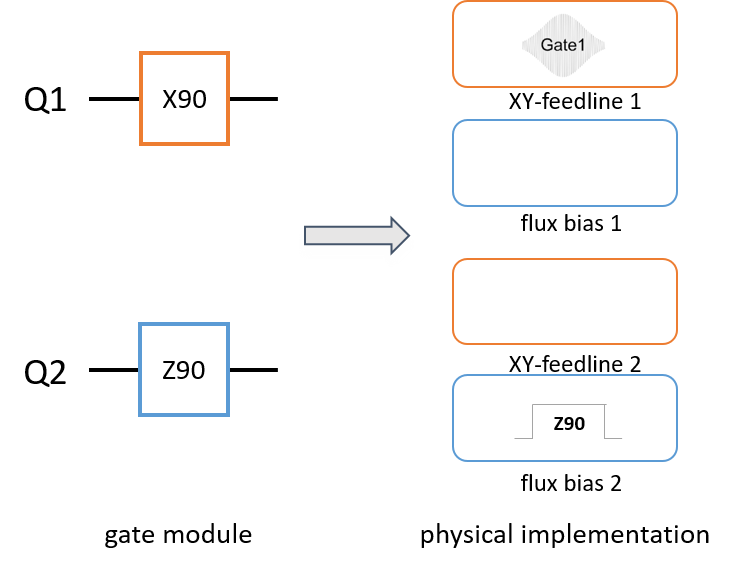
\includegraphics[width=2.2in]{3_1}
%   \caption{fig1}
%   \label{fig:side:a}
%   \end{minipage}%
%   \begin{minipage}[t]{0.5\textwidth}
%   \centering
%   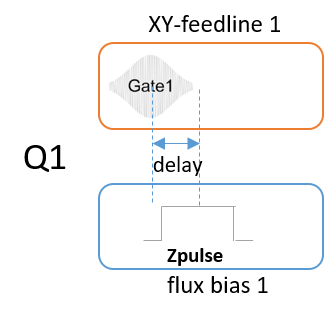
\includegraphics[width=2.2in]{3_4}
%   \caption{fig2}
%   \label{fig:side:b}
%   \end{minipage}
%   \end{figure*}
%   \begin{figure*}
%     \centering
%     \subfigure[Small Box with a Long Caption]{
%       \label{fig:subfig:a} %% label for first subfigure
%       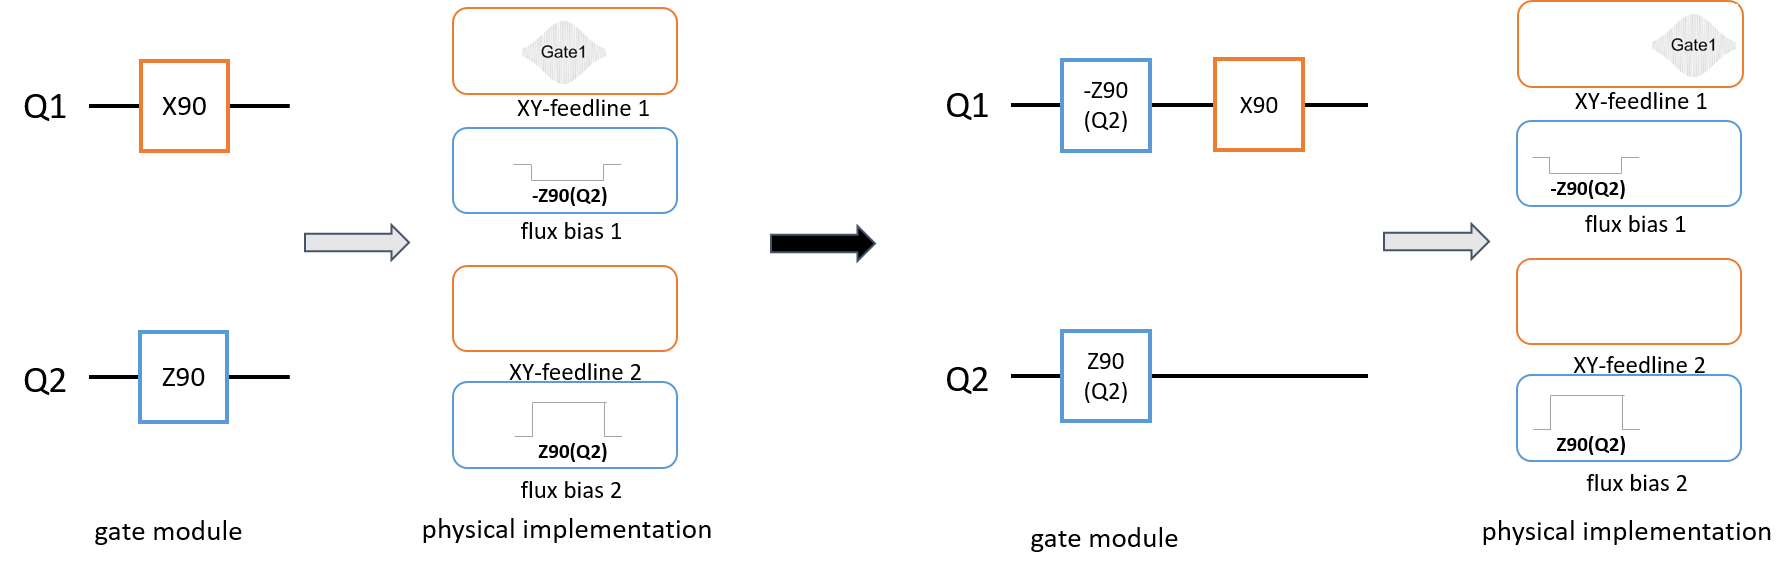
\includegraphics[width=\linewidth]{3_2}}
%     \subfigure[Big Box]{
%       \label{fig:subfig:b} %% label for second subfigure
%       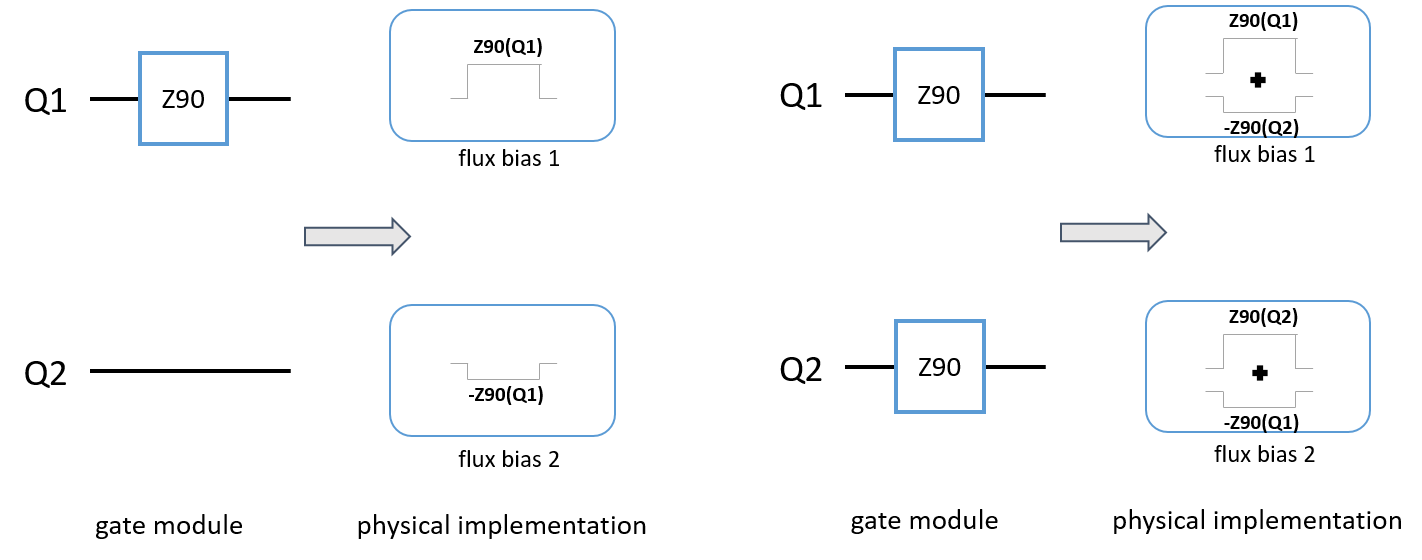
\includegraphics[width=\linewidth]{3_3}}
%     \caption{Two Subfigures}
%     \label{fig:subfig} %% label for entire figure
%   \end{figure*}



\subsection{Limitations Of The Gate Model}
\begin{figure}[ht]
  \centering
  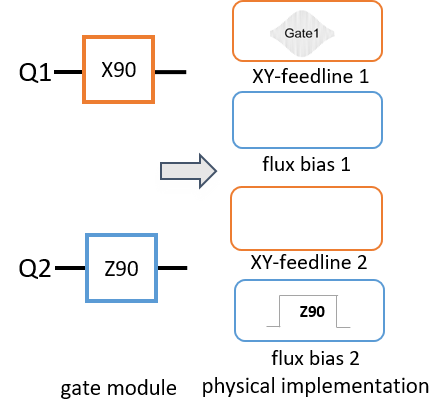
\includegraphics[width=\linewidth]{figure/2_1}
  \caption{The quantum circuit based on the gate model and physical implementation}
  \label{img2_1}
\end{figure}
At present, quantum programs are mainly divided into quantum algorithms and quantum experiments 
(such as RB, allXY), the basic unit of which are quantum gates. In the gate model of quantum computing, 
a program is typically decomposed into a sequence of 1and 2-qubit gates that are realized as control 
pulses acting on corresponding electrode, as shown in Figure~\ref{}. The left side of the figure is a gate model
description of a simple quantum circuit, and the right side is the control practical waveform applied by each 
electrode corresponding to the circuit.

Generally, the controller used to execute quantum programs adopts the gate model to describe 
the quantum program, which greatly reduces the memory consumption and uploading latency of waveform files, 
by combining quantum circuit with basic quantum gates at runtime.However, considering the physical limitations of quantum processors, 
as mentioned in Section 2, the quantum computing architecture requires to support waveform compensation and waveform paramater calibration, 
which is hard to be achieved by the gate model, poseing a challenge for quantum architecture design.

\begin{figure*}[ht]
  \centering
  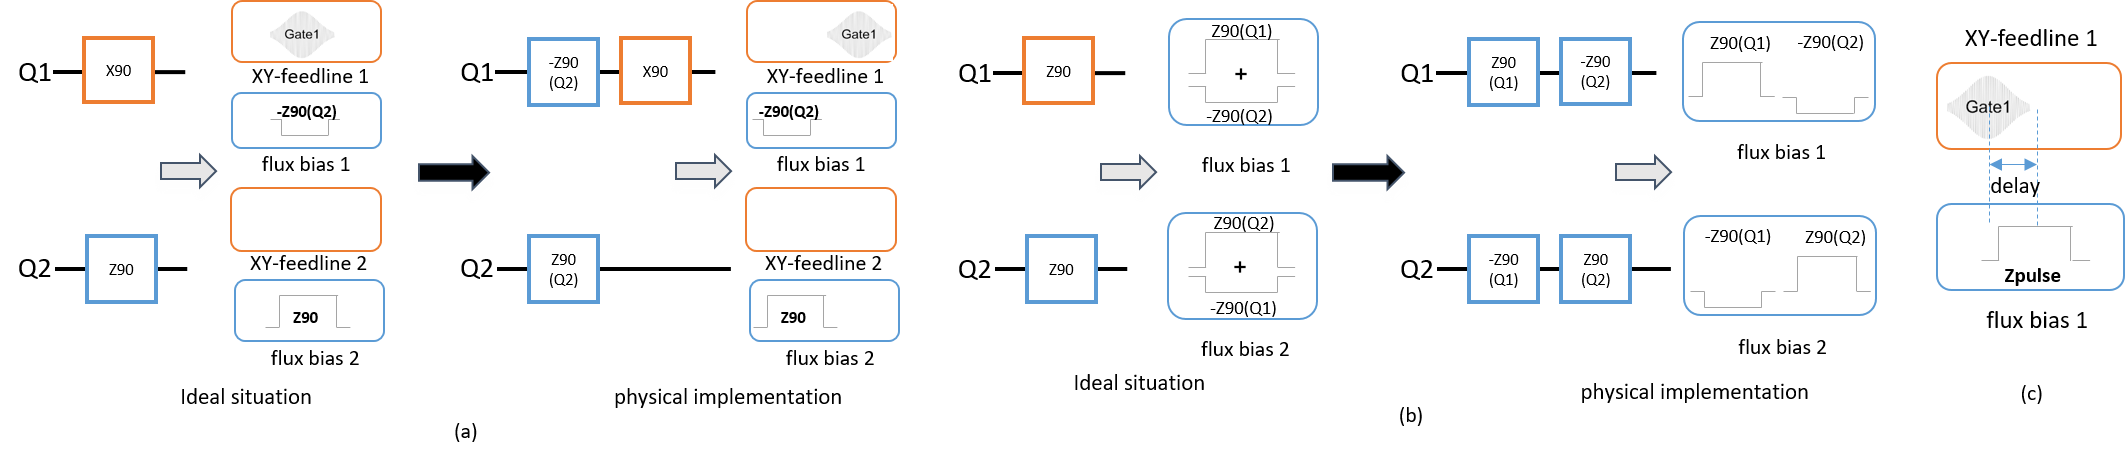
\includegraphics[width=\linewidth]{figure/2_2}
  \caption{Challenges of the gate model}
  \label{img2_2}
\end{figure*}


\subsubsection{Waveform compensation}
Using the gate model to implement waveform compensation increases instruction overhead and reduces the parallelism
of quantum circuits, which limit the scalability of the quantum architecture.

We first consider the case where there is only one compensation gate at one timestamp, 
as shown in Figure 3 (b). At this timestamp, X180 and Z180 are applied to Q1 and Q2, 
respectively. As the two electrodes of Q1 need to apply waveforms at the same time, 
it cannot be described by the gate model. One solution is to execute Z90 Q2 and X180 Q1 in sequence. 
However, it converts efficient parallel circuit into serial one, increasing the depth of circuit. 
On the other hand, when describing the Z180 Q2 in gate model, 
since the rest of qubits require to apply compensation waveforms simultaneously, 
the n-qubit quantum processor needs a total of n operation instructions to implement one compensation gate, 
which greatly increases the complexity of the circuit description and the number of basic logic gates.

For the case where multiple compensation gates are executed at one timestamp, 
as shown in Figure 3 (c), Q1 and Q2 applies Z180 simultaneously, 
since the waveform applied on Q1 is the superposition of the waveforms of Z180 Q1 and the compensation waveform of the Z180 Q2, 
it requires to two different quantum operations to encode Z180 Q1 gate. 
For n-qubit quantum processor, considering all combinations of m types of compensation gates performed at one timestamp, 
each qubit needs to store A waveforms of control operations and B of compensation operations. 
Obviously such a huge number of basic quantum gates are not scalable. 
Although the number of basic gates can be reduced at the cost of the depth of circuit, 
the n compensation gates that are executed simultaneously need to be transformed into n depth circuit, still unacceptable.

\subsubsection{Calibration experiment}
The gate model is not suitable for the description of certain calibration experiments, 
such as the delay calibration experiments between XY pulse and Z pulse. 
Since the latency between the transmission lines of qubits, fluctuating irregularly result from environment noise, 
reduces the fidelity of quantum gates, it is necessary to periodically calibrate the latency and modify the control waveform. 
The experimental waveform is shown in the figure 3 (d). 
The specific experimental scheme can refer to []. 
This experiment requires applying Z pulse and XY pulse to one qubit simultaneously and measuring the final state, contrary to the gate model. 
Therefore, a new circuit description scheme needs to be adopted at the microarchitecture level to support the quantum program execution flow as mentioned in Section1, 
which constitutes a challenge in the design of the quantum architecture.


\subsection{Description Of High Gate Diversity Circuit}
The current quantum programs can mainly divide into two categories: 
the first one is represented by RB algorithm, 
which is characterized by huge circuit depth but small gate density. 
Since the RB algorithm consists of a large number of subroutines, 
the depth of which can be as high as 2000, 
pre-storing all control waveforms will cause large memory overhead and transmission delay. 
Considering each RB program only performs quantum gates on 1-2 qubits, 
it is very suitable to use the gate model description, 
and play the pre-stored waveform of basic quantum gates according to the instructions in runtime.

The second type is used to solve practical problems which requires high-fidelity quantum gates, 
so the depth of circuit is relatively low, 
but the gate density and diversity depend on the specific algorithm.
When the gate diversity is high, it is inefficient to use the gate model. 
Specifically, it can cause serious timing problems when the time overhead of executing quantum 
operation instructions in microarchitecture is greater than the length of corresponding waveforms. 
Recent research has proposed double index quantum vector scheme which support SIMD (same gate, multiple qubits) 
and MIMD (multiple gates, multiple qubits) parallelism in a single instruction to increase the information density of quantum 
operation instructions, but introduces substantial complexity and hardware costs.

Therefore, a new circuit description scheme with satisfying performance for both type of circuits is another important challenge.

\begin{figure*}[ht]
  \centering
  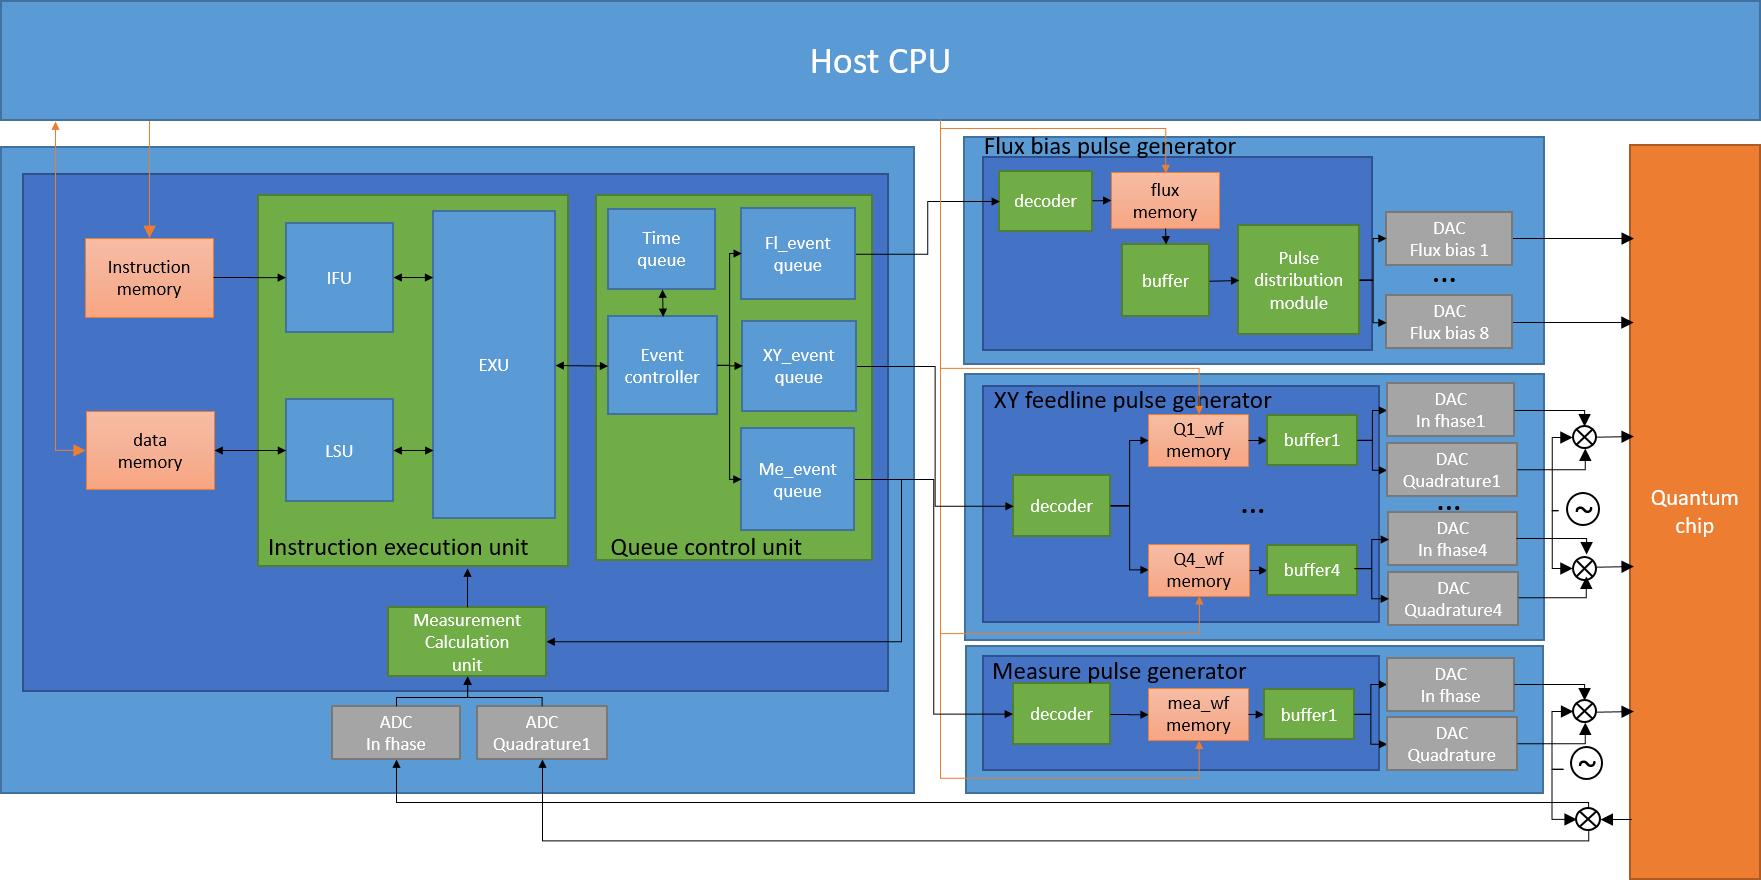
\includegraphics[width=\linewidth]{figure/4_1}
  \caption{overview of electrode event-based microarchitecture}
  \label{img2}
\end{figure*}